\documentclass[10pt,conference,a4paper]{IEEEtran}
\usepackage{ifpdf}

\ifCLASSINFOpdf
  \usepackage[pdftex]{graphicx}
  \DeclareGraphicsExtensions{.pdf,.jpeg,.png,.jpg}
\else
  \usepackage[dvips]{graphicx}
  \DeclareGraphicsExtensions{.eps}
\fi

\usepackage{amsmath,amsxtra,amssymb,amsthm,latexsym,amscd,amsfonts}
\usepackage[utf8]{vntex}
\usepackage{array}
\usepackage{epstopdf}
\usepackage{anysize}
\usepackage{subcaption}
\marginsize{2.4cm}{2.0cm}{3.2cm}{3.0cm}
\usepackage{balance}
\usepackage{cite}


% để cho công thức k bị ngắt dòng ngẫu nhiên
\relpenalty=10000
\binoppenalty=10000

\hyphenation{op-tical net-works semi-conduc-tor}


\begin{document}
\columnsep=0.63cm

\title{Phương pháp đánh giá kỹ thuật vũ đạo tự động dựa trên xử lý chuyển động và học máy}

\author{
\IEEEauthorblockN{
Vũ Mạnh Hiếu,
Trịnh Trung Kiên,
Bùi Quốc Huy,
Vũ Hữu Tiến
}
\IEEEauthorblockA{Học viện Công nghệ Bưu chính Viễn thông \\
Email: \{hieuvm.b23pt133, kientt.b23pt173\}@stu.ptit.edu.vn, \{tienvh, huybq\}@ptit.edu.vn}
}
\maketitle

\begin{abstract}
Việc tự rèn luyện vũ đạo qua video thường gặp khó khăn do người học thiếu sự phản hồi khách quan và kịp thời từ người hướng dẫn. Nhằm giải quyết vấn đề này, phương pháp đánh giá kỹ thuật vũ đạo được đề xuất để hỗ trợ quá trình tự rèn luyện của người học. Để khắc phục các hạn chế do bất đồng bộ thời gian và sai lệch tỉ lệ cơ thể, quy trình xử lý hai giai đoạn kết hợp giữa xử lý tín hiệu chuyển động và học máy được áp dụng. Cụ thể, các điểm khớp từ mô hình tư thế có độ tin cậy thấp bị loại bỏ và được bù bằng nội suy, sau đó tọa độ hai chiều được chuẩn hóa theo chiều dài thân hình. Tiếp đó, thuật toán DTW được sử dụng để căn chỉnh pha chuyển động giữa người học và video chuẩn. Trên các khung hình đã đồng bộ, hệ thống trích xuất sai số khoảng cách không gian, độ tương đồng hướng và sai số vận tốc để huấn luyện mô hình phân loại từng khớp, trước khi tổng hợp điểm số khung hình từ nhãn các khớp. Kết quả thực nghiệm cho thấy phương pháp đề xuất có khả năng nhận diện các khung hình sai kỹ thuật và chỉ ra chi tiết khớp mắc lỗi.
\end{abstract}

\begin{IEEEkeywords}
Đánh giá vũ đạo, ước lượng tư thế, DTW, xử lý dữ liệu khớp, học máy.
\end{IEEEkeywords}

\IEEEpeerreviewmaketitle

\section{GIỚI THIỆU}
\label{Sec:GioiThieu}

Việc nhảy đòi hỏi sự phối hợp chặt chẽ giữa mức độ chính xác của từng tư thế cơ thể và khả năng bắt đúng nhịp điệu theo thời gian \cite{Zhou_2021}. Trong phương thức giảng dạy truyền thống, các nhận xét và việc chỉnh sửa lỗi sai hoàn toàn phụ thuộc vào quan sát của người dạy. Cách tiếp cận này khó bảo đảm tính thống nhất trong các tiêu chí chấm điểm \cite{LAN2026200596}, đồng thời khiến người học gặp trở ngại nếu muốn tự rèn luyện tại nhà mà không có giáo viên trực tiếp kèm cặp.

Trong những năm gần đây, nhu cầu học nhảy ngày càng tăng, đặc biệt ở nhóm người trẻ, nhờ sức lan tỏa của các nền tảng mạng xã hội. Dù vậy, việc đăng ký học trực tiếp ở các trung tâm chuyên nghiệp thường kéo theo chi phí cao, bị ràng buộc bởi lịch học hoặc chịu ảnh hưởng bởi khoảng cách di chuyển \cite{kang2023dancing}. Vì thế, hình thức tự tập thông qua các video hướng dẫn trên mạng đang trở thành lựa chọn phổ biến \cite{hong2020youtube}. Tuy nhiên, phương thức tự học này bộc lộ nhiều hạn chế rõ rệt. Thứ nhất là nhận định mang tính chủ quan. Khi người học tự quan sát qua gương hoặc tự quay video, việc đánh giá mình nhảy đã đúng chuẩn hay chưa trở nên rất khó, từ đó dễ lặp lại các động tác sai một cách thường xuyên, hình thành thói quen khó khắc phục \cite{Zhou_2021}. Thứ hai, về rào cản chi phí, các buổi kèm riêng với người dạy có chuyên môn thường ở mức học phí khá cao, khiến nhiều người mới bắt đầu không thể duy trì việc học trong thời gian dài. Thứ ba là việc thiếu phản hồi kịp thời, khi chỉ xem video theo một chiều, người học không biết sai ở điểm nào, cũng như mức độ tiến bộ ra sao, nên dễ nản và có thể bỏ cuộc giữa chừng.

Từ thực trạng đó, việc phát triển một công cụ hỗ trợ tự luyện tập có khả năng phát hiện lỗi sai một cách khách quan và tức thì là hết sức cần thiết. Dù vậy, để thực hiện điều này trên máy tính, chúng ta phải giải quyết các thách thức kỹ thuật đáng kể. Đầu tiên, người học thường nhảy nhanh hơn hoặc chậm hơn so với video mẫu, dẫn tới việc lệch pha thời gian, khiến việc đối chiếu trực tiếp theo từng giây và từng khung hình không thể áp dụng \cite{article}. Ngoài ra, mỗi người có chiều cao, độ dài tay chân khác nhau, đồng thời đứng gần hay xa camera cũng không giống nhau, do đó hệ thống cần chuẩn hóa dữ liệu về cùng một tỷ lệ trước khi tiến hành so khớp. Bên cạnh đó, kết quả đánh giá không nên chỉ là một điểm số chung mà cần chỉ ra khớp nào sai để người học biết cần sửa ở đâu. Nhằm giải quyết những thách thức kỹ thuật đó, bài báo đề xuất một phương pháp đánh giá kỹ thuật vũ đạo tự động dựa trên xử lý chuyển động và học máy. Mục tiêu của nghiên cứu là cung cấp một phương pháp đánh giá khách quan, giúp người học biết mình đã nhảy đúng động tác hay chưa, từ đó chủ động chỉnh sửa.

Đóng góp chính của bài báo này bao gồm:
\begin{itemize}
    \item Kết hợp căn chỉnh thời gian và đánh giá độ chuẩn xác của tư thế: căn chỉnh bằng DTW cho phép so sánh tư thế bất kể tốc độ thực hiện, và từng khớp được phân loại chi tiết. Phương pháp là nền tảng để mở rộng sang đánh giá nhịp điệu trong các nghiên cứu tiếp theo.
    \item Cơ chế chấm điểm hai tầng có tính giải thích: hệ thống sử dụng mô hình học máy để phân loại từng khớp, sau đó tổng hợp nhãn các khớp để xác định khung hình đạt hay không; điều này giúp người học nhận biết chính xác mình sai ở đâu để chỉnh sửa.
    \item Bài báo đề xuất cơ chế tổng hợp điểm khung hình từ nhãn từng khớp và chọn ngưỡng bằng grid search với ràng buộc Recall Fail $\geq$ 0.90.
\end{itemize}

Phần còn lại của bài báo được bố cục như sau: Phần II trình bày về các nghiên cứu liên quan đến bài toán; Phần III đề xuất phương pháp đánh giá cho bài toán; Phần IV mô tả thiết lập thực nghiệm và phân tích các kết quả đạt được; cuối cùng, Phần V đưa ra kết luận và hướng phát triển trong tương lai.

\section{CÁC NGHIÊN CỨU LIÊN QUAN}
\label{Sec:BaiBaoLienQuan}

Một hướng tiếp cận phổ biến trong những năm gần đây để đánh giá động tác dựa trên thị giác máy tính và trí tuệ nhân tạo là sử dụng Human Pose Estimation để trích xuất các điểm khớp hoặc biểu diễn bộ xương người từ video, sau đó sử dụng các đặc trưng không gian và thời gian để đánh giá chất lượng chuyển động \cite{THARATIPYAKUL2024e36589}.

Wang và Ngoi \cite{wang2023dance} đã đề xuất hệ thống Dancing Mirror, trong đó sử dụng mô hình trích xuất landmark cơ thể theo thời gian thực từ webcam và đối chiếu với video tham chiếu đã được quay trước. Điểm nổi bật của giải pháp này là khả năng cung cấp phản hồi trực quan ngay trên màn hình hiển thị, giúp người tập nhận biết nhanh các sai lệch tư thế thông qua ngưỡng chênh lệch góc khớp, và đã được thử nghiệm trên người học ở mức mới bắt đầu và trung cấp. Tuy vậy, tác giả ghi nhận hạn chế khi dùng phim phản chiếu dán lên màn hình để tạo hiệu ứng gương: người dùng phải đứng xa (khoảng 5 mét) mới nhìn rõ nên khó đọc được phản hồi trên giao diện, đồng thời nghiên cứu không đề cập đến việc căn chỉnh thời gian giữa chuyển động của người tập và video tham chiếu, nên chưa giải quyết được vấn đề lệch nhịp khi người dùng nhảy liên tục xuyên suốt cả một bài.


Nhằm xử lý độ lệch pha thời gian, Effendi và cộng sự \cite{effendi2023} đã kết hợp MediaPipe với thuật toán Dynamic Time Warping (DTW) để đánh giá điệu múa truyền thống Tari Remo. Phương pháp này đối chiếu thành công chuỗi chuyển động của người học với video mẫu và cảnh báo khi góc cử động bị sai lệch. Tuy nhiên, nghiên cứu mới chỉ đối chiếu các góc khớp với ngưỡng cố định, chưa khai thác các đặc trưng động học (kinematic features) đa chiều và thiếu mô hình học máy để phân loại độ nhạy lỗi sai. Đồng thời, việc chưa chuẩn hóa dữ liệu theo thân người khiến kết quả dễ bị ảnh hưởng bởi cự ly và góc quay camera.

Trong bối cảnh bảo tồn nghệ thuật múa truyền thống, Siswoyo \cite{siswoyo2026} đã triển khai mô hình MediaPipe kết hợp thư viện OpenCV để đánh giá các động tác cơ bản. Nghiên cứu này có ưu điểm ở chỗ sử dụng khoảng cách Euclidean giữa tọa độ tư thế người tập và tư thế tham chiếu để phân loại động tác đúng hoặc sai. Tuy nhiên, độ chính xác giảm rõ rệt khi ánh sáng yếu, khi người múa thực hiện động tác nhanh hoặc khi cơ thể bị che khuất một phần.

Nhìn chung, các nghiên cứu trước đây đã ghi nhận tính khả thi của việc đánh giá động tác từ mốc xương khớp thu được từ camera. Tuy nhiên, những phương pháp này vẫn còn một số hạn chế nhất định. Trước hết, việc xử lý lệch nhịp thời gian giữa hai video bài nhảy vẫn chưa triệt để, trong khi cách tiếp cận gom cụm các tư thế ảnh tĩnh lại làm mất đi tính liên tục của chuỗi động tác. Bên cạnh đó, tọa độ chiều sâu $Z$ do mô hình ước tính từ camera 2D thông thường dễ bị nhiễu.

Để khắc phục các điểm yếu này, bài báo đề xuất quy trình kết hợp. Đầu tiên, loại bỏ dữ liệu trục $Z$ vốn dễ nhiễu, chuyển tọa độ về mặt phẳng hai chiều và chuẩn hóa theo chiều dài thân người, đồng thời sử dụng thuật toán DTW \cite{article} nhằm căn chỉnh thời gian giữa hai chuỗi động tác. Sau đó, hệ thống trích xuất đồng thời độ lệch về vị trí, hướng và vận tốc của từng khớp để huấn luyện mô hình phân loại, trước khi tổng hợp điểm cho từng khung hình từ nhãn của các khớp.

\section{PHƯƠNG PHÁP ĐỀ XUẤT}
\label{Sec:PhuongPhapDeXuat}

Kiến trúc tổng thể của hệ thống được mô tả chi tiết trong Hình \ref{fig:pipeline}.
\begin{figure*}[!t]
    \centering
    \includegraphics[width=0.8\linewidth]{pipeline.png}
    \caption{Sơ đồ quy trình tổng quan của hệ thống đánh giá động tác.}
    \label{fig:pipeline}
\end{figure*}
\subsection{Tiền xử lý và chuẩn hóa giải phẫu}
Dữ liệu tọa độ 3D từ MediaPipe \cite{lugaresi2019mediapipe} thường gặp hiện tượng mất dấu và dao động bất ổn định giữa các khung hình. Quá trình tiền xử lý bao gồm hai bước: tái tạo tín hiệu và chuẩn hóa không gian \cite{lepot2017interpolation}. Ngoài ra, để loại bỏ nhiễu tĩnh ngay từ đầu, các video học viên có độ lệch chuẩn chuyển động trung bình trên 4 khớp ngọn (cổ tay trái/phải và cổ chân trái/phải) nhỏ hơn $0.020$ sẽ bị loại tự động khỏi tập dữ liệu.

Đầu tiên, ở bước tái tạo tín hiệu, các điểm khớp có chỉ số $\text{Visibility} < 0.5$, cho thấy điểm khớp có thể bị che khuất hoặc khó nhận diện trong ảnh, được gán giá trị thiếu (NaN) và được phục hồi bằng phương pháp nội suy tuyến tính dựa trên các khung hình liền kề nhằm đảm bảo tính liên tục của quỹ đạo. Ở bước chuẩn hóa không gian 2D, do camera thông thường không có cảm biến độ sâu và trục $Z$ ước tính kém ổn định, hệ thống loại bỏ trục $Z$ và dời gốc tọa độ $(0,0)$ về trung điểm của hông:
\begin{equation}
\mathbf{p}_{Root} = \left( \frac{X_{L\_Hip} + X_{R\_Hip}}{2}, \frac{Y_{L\_Hip} + Y_{R\_Hip}}{2} \right)
\end{equation}
Trong đó $(X_{L\_Hip}, Y_{L\_Hip})$ và $(X_{R\_Hip}, Y_{R\_Hip})$ lần lượt là tọa độ 2D của khớp hông trái và hông phải.

Chiều dài thân người ($Torso$) được đo bằng khoảng cách Euclidean giữa trung điểm hai vai $\mathbf{p}_{Sh} = (X_{Sh}, Y_{Sh})$, với $X_{Sh} = (X_{L\_Sh} + X_{R\_Sh})/2$ và $Y_{Sh} = (Y_{L\_Sh} + Y_{R\_Sh})/2$, và gốc hông $\mathbf{p}_{Root} = (X_{Root}, Y_{Root})$. Đặt $d_X = X_{Sh} - X_{Root}$ và $d_Y = Y_{Sh} - Y_{Root}$:
% \begin{equation}
% \begin{aligned}
% Torso = \max\Bigg(
% &\sqrt{(X_{Sh}-X_{Root})^2
%       +(Y_{Sh}-Y_{Root})^2},\\
% &\quad 10^{-5}
% \Bigg).
% \end{aligned}
% \label{eq:torso}
% \end{equation}

\begin{equation}
Torso = \max\left(\sqrt{d_X^{2} + d_Y^{2}},\ 10^{-5}\right)
\label{eq:torso}
\end{equation}

Tọa độ của từng khớp $i$ sau đó được chia theo tỷ lệ thân người để giảm sự khác biệt về chiều cao hay khoảng cách đứng tới camera:
\begin{equation}
\hat{X}^{(i)} = \frac{X^{(i)} - X_{Root}}{Torso}, \quad \hat{Y}^{(i)} = \frac{Y^{(i)} - Y_{Root}}{Torso}
\end{equation}
Với $i \in \{1, \dots, 13\}$ tương ứng với 13 khớp giải phẫu chủ đạo bao gồm: 01 điểm mốc định vị đầu (mũi), 06 khớp chi trên (vai, khuỷu tay, cổ tay trái/phải), cùng 06 khớp thân dưới và chi dưới (hông, đầu gối, cổ chân trái/phải). Thay vì sử dụng toàn bộ các landmarks, nghiên cứu lựa chọn 13 điểm có vai trò đại diện cho đầu, thân, chi trên và chi dưới.

\subsection{Đồng bộ thời gian và trích xuất đặc trưng}
Do tốc độ thực hiện động tác của học viên và giáo viên không đồng đều, hệ thống sử dụng thuật toán FastDTW \cite{salvador2007fastdtw} (xấp xỉ của Dynamic Time Warping \cite{sakoe1978dtw}) với khoảng cách Euclidean để tìm đường căn chỉnh tối ưu giữa hai chuỗi khung hình \cite{article}. Nếu một khung hình của học viên được căn chỉnh với nhiều khung hình mẫu thì các cặp đó đều được đưa vào tính toán. Sau khi đồng bộ, hệ thống trích xuất 3 đặc trưng cốt lõi cho phân tích học máy:
\begin{itemize}
    \item Đặc trưng không gian (Joint Error): Sai số biên độ vị trí tuyệt đối
\begin{equation}
Error = \sqrt{(X_s - X_t)^2 + (Y_s - Y_t)^2}
\end{equation}
Trong đó $(X_s, Y_s)$ và $(X_t, Y_t)$ là tọa độ chuẩn hóa $(\hat{X}, \hat{Y})$ của cùng một điểm khớp tương ứng của người học và giáo viên tại cặp khung hình đã đồng bộ qua DTW.
    \item Đặc trưng hướng (Joint Cosine): Độ tương đồng cosine giữa vector từ gốc hông tới khớp của học viên ($s$) và của giáo viên ($t$); giá trị càng gần $1$ thì hướng càng giống nhau.
\begin{equation}
Cosine = \frac{X_s X_t + Y_s Y_t}{\sqrt{X_s^2 + Y_s^2} \sqrt{X_t^2 + Y_t^2} + 10^{-9}}
\end{equation}
    \item Đặc trưng động học (Velocity Error): Sai số vận tốc. Vận tốc cục bộ tại khung hình $k$ của chuỗi đã căn chỉnh được ước lượng bằng sai phân bậc nhất $\Delta X = X^{(k)} - X^{(k-1)}$ và $\Delta Y = Y^{(k)} - Y^{(k-1)}$. Độ lệch vector vận tốc:
\begin{equation}
Vel\_Error = \sqrt{(\Delta X_s - \Delta X_t)^2 + (\Delta Y_s - \Delta Y_t)^2}
\end{equation}
\end{itemize}

\subsection{Đánh giá cấp độ khung hình \& Tối ưu ngưỡng}

Đầu tiên là việc phân loại theo cấp độ khớp. Do dữ liệu đặc trưng có mối quan hệ phức tạp và dễ bị ảnh hưởng bởi nhiễu từ thiết bị, hệ thống sử dụng các thuật toán boosting dựa trên nhóm cây quyết định để huấn luyện mô hình phân loại nhị phân; CatBoost \cite{prokhorenkova2018catboost} được lựa chọn sau khi so sánh ở Mục IV-B.
Mô hình tiếp nhận ma trận đầu vào gồm 3 biến liên tục $[Error, Cosine, Vel\_Error]$ và xuất ra nhãn dự đoán cho từng khớp là ĐÚNG (1) hoặc SAI (0).

Điểm của một khung hình $S_{frame}$ được tính bằng tổng các nhãn khớp dự đoán $P_i$, với các khớp có vai trò như nhau:
\begin{equation}
S_{frame} = \sum_{i=1}^{13} P_i
\end{equation}
Việc gán trọng số khác nhau cho từng bộ phận là hướng mở rộng của nghiên cứu.

Khung hình được xếp loại PASS nếu $S_{frame} \ge T$. Để xác định ngưỡng quyết định tối ưu $T^*$, phương pháp Grid Search được sử dụng trên dải giá trị $T \in [6.0, 8.9]$ với bước nhảy $0.1$. Hàm mục tiêu là tìm ngưỡng $T^*$ phân tách khung hình thành PASS/FAIL sao cho tối đa hóa chỉ số trung bình điều hòa $F1_{macro}$, dưới ràng buộc $Recall_{Fail} \ge 0.90$ (tỷ lệ bỏ sót khung hình múa sai dưới 10\%). Do $S_{frame}$ chỉ nhận giá trị nguyên nên các ngưỡng $T$ nằm trong cùng một khoảng cho kết quả phân loại như nhau. Ngưỡng $T^*$ được tối ưu hoàn toàn trên tập kiểm định (Validation) độc lập, sau đó giữ cố định khi đánh giá trên tập kiểm thử (Test) nhằm loại bỏ hoàn toàn hiện tượng rò rỉ dữ liệu (\textit{data leakage}).

\section{THIẾT LẬP THỰC NGHIỆM VÀ KẾT QUẢ}
\label{Sec:ThietLapVaKetQua}

\subsection{Tập dữ liệu và kiểm định tái tạo tín hiệu nội suy}
Tập dữ liệu ban đầu gồm 13 cặp video (học viên và video mẫu) được thu thập từ TikTok, thuộc nhiều thể loại nhảy khác nhau. Mỗi video có một người nhảy và được quay bằng nhiều loại thiết bị khác nhau. Sau bước lọc nhiễu tĩnh tự động ở Phase 1 ($\text{std} < 0.020$), một video học viên gần như đứng yên (Video 6, $\text{std} = 0.0193$) bị loại bỏ, giữ lại 12 cặp video hợp lệ. Các video được xử lý bằng MediaPipe để thu 13 điểm khớp trên mỗi khung hình. Nhãn do hai thành viên của nhóm tác giả gán thủ công ở mức khớp: khớp sai nghiêm trọng so với video mẫu được gán 0 (sai); các khớp còn lại được gán 1 (đúng), kể cả khi có lệch nhẹ nhưng không ảnh hưởng đến tính liền mạch và tổng thể của động tác. Nhãn khung hình được lấy theo đa số: khung hình là đúng nếu có ít nhất 7/13 khớp được gán 1.

Để loại bỏ hoàn toàn rò rỉ dữ liệu, 12 cặp video hợp lệ được phân chia theo cấp độ nhóm (\text{Video\_ID}) thành 3 tập độc lập:
\begin{itemize}
    \item \text{Tập huấn luyện (Train):} Gồm 8 cặp video (\text{[1, 2, 4, 8, 10, 11, 12, 15]}), cung cấp $4.544$ khung hình tương ứng với $60.190$ mẫu khớp đã đồng bộ DTW ($50{,}8\%$ Pass và $49{,}2\%$ Fail).
    \item \text{Tập kiểm định (Validation):} Gồm 2 cặp video (\text{[3, 7]}), cung cấp $892$ khung hình tương ứng với $12.090$ mẫu khớp ($57{,}7\%$ Pass và $42{,}3\%$ Fail), chỉ sử dụng để tìm ngưỡng tối ưu $T^*$.
    \item \text{Tập kiểm thử độc lập (Test):} Gồm 2 cặp video (\text{[5, 9]}), cung cấp $613$ khung hình tương ứng với $8.047$ mẫu khớp ($64{,}3\%$ Pass và $35{,}7\%$ Fail), hoàn toàn tách biệt trong quá trình huấn luyện và chọn ngưỡng.
\end{itemize}

Để kiểm chứng khâu nội suy, thực nghiệm che khuất nhân tạo được tiến hành trên hai khớp đại diện: khớp đầu gối phải (chi dưới) và khớp khuỷu tay trái (chi trên). Với mỗi khớp, nhóm lấy 100 khung hình có độ tin cậy cao ($\text{Visibility} > 0.95$), thay thế ngẫu nhiên 15\% số khung hình bằng giá trị thiếu (NaN) rồi áp dụng nội suy tuyến tính để tái lập quỹ đạo. Sai số được tính trên các điểm bị xóa và thực hiện một lần chạy. 
\text{Ground Truth ($X_{\text{original}}$):} Tọa độ $X$ chuẩn hóa ban đầu được trích xuất từ video của học viên tại các frame có độ tin cậy nhận diện cao (Visibility $> 0.95$), được sử dụng làm giá trị tham chiếu (ground truth).
\text{Interpolated ($X_{\text{interpolated}}$):} Tọa độ $X$ sau khi áp dụng thuật toán nội suy tuyến tính (\textit{linear interpolation}) nhằm khôi phục các vị trí bị thiếu do quá trình giả lập mất dấu, trong đó ngẫu nhiên $15\%$ số frame được loại bỏ.

Kết quả được thể hiện trong Hình~\ref{fig:interpolation_eval}. Cụ thể, khớp đầu gối phải đạt $\text{RMSE} = 0.0130$ và $\text{MAE} = 0.0107$; khớp khuỷu tay trái - có biên độ vung tay và biến thiên vận tốc lớn hơn - đạt $\text{RMSE} = 0.0292$ và $\text{MAE} = 0.0165$ (trên tọa độ $X$ thuộc khoảng $[0,1]$ của ảnh). Dạng sóng nội suy bám sát quỹ đạo gốc, cho thấy nội suy tuyến tính phục hồi các điểm mất dấu rời rạc với sai số thấp; sai lệch rõ hơn ở các đoạn chuyển động nhanh.
\begin{figure*}[!t]
    \centering

    \begin{subfigure}[b]{0.49\textwidth}
        \centering
        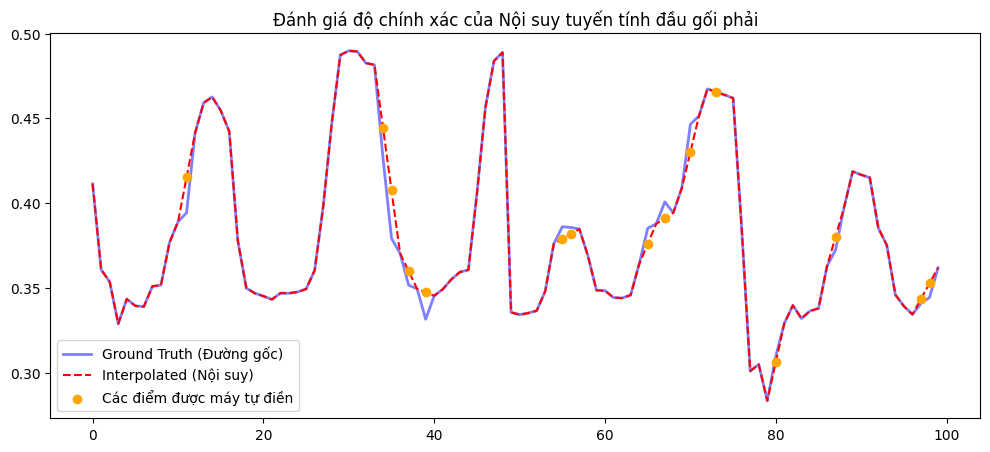
\includegraphics[width=\linewidth]{interp_knee.png}
        \caption{Khớp đầu gối phải}
        \label{fig:interp_knee}
    \end{subfigure}
    \hfill
    \begin{subfigure}[b]{0.49\textwidth}
        \centering
        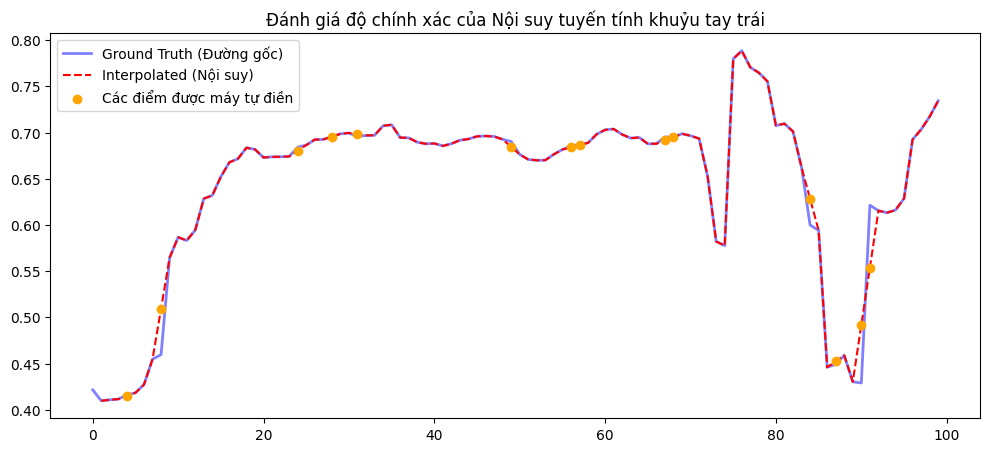
\includegraphics[width=\linewidth]{interp_elbow.png}
        \caption{Khớp khuỷu tay trái}
        \label{fig:interp_elbow}
    \end{subfigure}

    \caption{Đánh giá phương pháp nội suy tuyến tính
    trên tọa độ $X$ của hai khớp đại diện cho chi dưới và chi trên
    khi mất ngẫu nhiên 15\% khung hình.}
    \label{fig:interpolation_eval}
\end{figure*}
\subsection{Đánh giá đa mô hình cấp độ khớp}
Nhằm phân loại tính chính xác của động tác ở cấp độ từng khớp giải phẫu, bảy thuật toán học máy đơn lẻ (KNN, Decision Tree, Random Forest, XGBoost, LightGBM, CatBoost, Gradient Boosting) và một mô hình kết hợp (Ensemble) đã được đưa vào so sánh thực nghiệm trên ba đặc trưng cốt lõi: $\text{Joint\_Error}$, $\text{Joint\_Cosine}$ và $\text{Velocity\_Error}$. Các mô hình được huấn luyện trên tập huấn luyện và đánh giá trên tập kiểm thử. Kết quả so sánh chi tiết được trình bày trong Bảng~\ref{tab:tong_hop_mo_hinh}.

\begin{table*}[!t]
    \centering
    \caption{Tổng hợp so sánh hiệu năng phân loại cấp khớp và tốc độ của các mô hình (CatBoost: 100 vòng lặp, độ sâu 6, tốc độ học 0.1)}
    \label{tab:tong_hop_mo_hinh}
    \resizebox{\textwidth}{!}{%
    \begin{tabular}{lccccc}
        \hline
        \textbf{Mô hình}
        & \textbf{Độ chính xác (\%)} & \textbf{Macro F1} & \textbf{Thời gian huấn luyện (s)} & \textbf{Độ trễ/khung (ms)} & \textbf{FPS}\\
        \hline
        K-Nearest Neighbors (KNN)   & 61.28 & 0.6037 & 0.078  & 1.2400 & 806   \\
        Decision Tree               & 71.87 & 0.7042 & 0.259  & 0.5856 & 1708 \\
        Random Forest               & 73.84 & 0.7206 & 7.021  & 2.5587 & 391   \\
        XGBoost                     & 72.76 & 0.7108 & 1.672  & 1.0097 & 990   \\
        LightGBM                    & 73.48 & 0.7174 & 2.029  & 1.3333 & 750   \\
        \textbf{CatBoost}           & 74.15 & 0.7235 & 0.782 & 0.4892 & 2044 \\
        Gradient Boosting           & 74.46 & 0.7249 & 21.516 & 0.4652 & 2150 \\
        Ensemble (Soft Voting)      & 73.59 & 0.7181 & 34.690 & 18.5759 & 54   \\
        \hline
    \end{tabular}%
    }
\end{table*}

Số liệu từ Bảng~\ref{tab:tong_hop_mo_hinh} cho thấy các mô hình thuộc nhóm cây (Tree-based ensemble) cho kết quả cao hơn so với thuật toán dựa trên khoảng cách hình học. K-Nearest Neighbors ($\text{KNN}$) cho hiệu năng thấp nhất với độ chính xác $61.28\%$ và Macro F1-score $0.6037$, gợi ý rằng ranh giới phân lớp của sai số động học khó phân tách chỉ bằng các thước đo khoảng cách đồng nhất.

Trong các kiến trúc Boosting, chênh lệch về độ chính xác và Macro F1 giữa Gradient Boosting, CatBoost, LightGBM và XGBoost là nhỏ (dưới $2\%$). Với một lần chia dữ liệu và tập kiểm thử chỉ gồm hai video, sự chênh lệch này chưa đủ để kết luận mô hình nào tốt hơn. Tuy nhiên, CatBoost \cite{prokhorenkova2018catboost} chỉ mất $0.782$ giây để huấn luyện - nhanh hơn khoảng $27$ lần so với Gradient Boosting ($21.516$ giây). Bên cạnh đó, nhằm kiểm chứng khả năng vượt qua giới hạn của các mô hình đơn lẻ, cơ chế ensemble learning theo phương pháp Soft Voting cũng được triển khai \cite{zhou2012ensemble}. Soft Voting đưa ra phán quyết cuối cùng bằng cách tính trung bình cộng xác suất dự đoán từ các mô hình thành phần. Tuy nhiên, việc kết hợp này không cải thiện Macro F1-score ($0.7181$) mà còn làm tăng thời gian huấn luyện lên đáng kể ($34.690$ giây). Do đó, CatBoost được lựa chọn làm bộ phân loại cấp khớp nhờ hiệu năng tương đương các mô hình tốt nhất cùng chi phí huấn luyện thấp. Phân tích mức độ quan trọng đặc trưng trên CatBoost cho thấy sai số vị trí không gian $\text{Joint\_Error}$ đóng vai trò chủ đạo với tỷ trọng $50{,}67\%$, tiếp theo là độ tương đồng hướng $\text{Joint\_Cosine}$ đạt $27{,}27\%$ và sai số vận tốc $\text{Velocity\_Error}$ chiếm $22{,}06\%$, khẳng định vai trò bổ trợ thiết yếu của cả ba nhóm đặc trưng động học.

\subsection{Quyết định cấp độ khung hình và chọn ngưỡng}

Phương pháp tổng hợp điểm trên toàn khung hình sử dụng các khớp với vai trò như nhau. Để xác định ngưỡng phán quyết tối ưu $T^*$, hệ thống thực hiện quét tham số (Grid Search) trên dải giá trị $T \in [6.0, 8.9]$ với bước nhảy $0.1$ hoàn toàn trên \text{tập kiểm định độc lập (\text{Videos [3, 7]}, $892$ khung hình)}.

Do tổng điểm khung hình $S_{frame}$ chỉ nhận giá trị nguyên từ $0$ đến $13$, các ngưỡng nằm trong cùng một khoảng đơn vị cho kết quả phân loại tương đương nhau. Dưới điều kiện ràng buộc duy trì độ nhạy bắt lỗi $Recall_{Fail} \ge 0.90$ nhằm hạn chế bỏ sót động tác sai kỹ thuật, quá trình Grid Search trên tập Validation xác định ngưỡng tối ưu tại $T^* = 8.1$ (tương đương yêu cầu ít nhất $9/13$ khớp được phân loại đúng, $S_{frame} \ge 9$). Tại mốc ngưỡng này, mô hình đạt độ chính xác $\text{Validation Accuracy} = 70{,}29\%$ và $\text{Validation Macro-F1} = 0{,}6033$. Sau khi xác lập trên tập kiểm định, ngưỡng $T^* = 8.1$ được khóa cố định để đánh giá khách quan trên tập kiểm thử độc lập ở Mục IV-D, loại bỏ hoàn toàn nguy cơ rò rỉ dữ liệu.
\subsection{Kết quả thực nghiệm}

\begin{table*}[!t]
    \centering
    \caption{Báo cáo chi tiết hiệu năng đánh giá cấp độ khung hình của mô hình CatBoost trên tập kiểm thử (Ngưỡng cố định $T^* = 8.1$)}
    \label{tab:frame_classification_report}
    \setlength{\tabcolsep}{10pt}
    \renewcommand{\arraystretch}{1.15}
    \begin{tabular}{lcccc}
        \hline
        \textbf{Nhãn phân loại} & \textbf{Precision} & \textbf{Recall} & \textbf{F1-score} & \textbf{Số lượng} \\
        \hline
        Fail (0)                & 0.84 & 0.90 & 0.87 & 203 \\
        Pass (1)                & 0.95 & 0.91 & 0.93 & 410 \\
        \hline
        \textbf{Độ chính xác} & \multicolumn{3}{c}{\textbf{90.86\%}} & \textbf{613} \\
        Macro Avg               & 0.89 & 0.91 & 0.90 & 613 \\
        Weighted Avg            & 0.91 & 0.91 & 0.91 & 613 \\
        \hline
    \end{tabular}
\end{table*}

\begin{table*}[!t]
    \centering
    \caption{Ma trận nhầm lẫn trên 613 khung hình kiểm thử độc lập ($T^*=8.1$)}
    \label{tab:confusion_matrix}
    \setlength{\tabcolsep}{10pt}
    \renewcommand{\arraystretch}{1.2}
    \begin{tabular}{lcc}
        \hline
        \textbf{Thực tế \textbackslash{} Dự đoán} & \textbf{Dự đoán FAIL (0)} & \textbf{Dự đoán PASS (1)} \\
        \hline
        \textbf{Thực tế FAIL (0)}  & 183 (True Negative)       & 20 (False Positive)       \\
        \textbf{Thực tế PASS (1)}  & 36 (False Negative)       & 374 (True Positive)       \\
        \hline
    \end{tabular}
\end{table*}

Nghiên cứu sử dụng các tham số trích xuất từ ma trận nhầm lẫn (Confusion Matrix) bao gồm: \text{True Positive} (TP), \text{True Negative} (TN), \text{False Positive} (FP) và \text{False Negative} (FN), với lớp PASS là lớp dương. Từ các tham số cơ sở này, hiệu năng của mô hình được tính toán thông qua bốn độ đo: Độ chính xác tổng thể (\text{Accuracy}), độ chuẩn xác (\text{Precision}), độ nhạy (\text{Recall}) và điểm F1 (\text{F1-score}) \cite{SOKOLOVA2009427}. Đối với bài toán này, chỉ số độ nhạy trên lớp lỗi ($Recall_{Fail}$) được sử dụng để xác định tỷ lệ bỏ lọt các động tác sai kỹ thuật.

Hiệu năng chi tiết trên tập kiểm thử độc lập được thể hiện ở Bảng~\ref{tab:frame_classification_report} và Bảng~\ref{tab:confusion_matrix}. Tại ngưỡng cố định $T^* = 8.1$, mô hình CatBoost đạt độ chính xác tổng thể $90{,}86\%$ và $\text{Macro-F1} = 0{,}8988$ trên $613$ khung hình kiểm thử, vượt trội đáng kể so với mức cơ sở luôn dự đoán lớp đa số PASS ($66{,}88\%$). Kết quả ma trận nhầm lẫn ghi nhận $TN = 183$ khung hình lỗi được nhận diện chính xác và $TP = 374$ khung hình đúng được phân loại chuẩn xác.

Chỉ số độ nhạy đối với lớp lỗi đạt $Recall_{Fail} = 90{,}15\%$ ($183/203$), trong khi độ nhạy lớp đúng đạt $Recall_{Pass}=91{,}22\%$ ($374/410$), cho thấy sự cân bằng cao giữa khả năng phát hiện lỗi và tránh phạt nhầm người học. Về các trường hợp dự đoán sai, chỉ có $20$ khung hình lỗi bị bỏ lọt thành đúng ($FP = 20$, chiếm $3{,}26\%$ tổng khung hình) và $36$ khung hình đúng bị đánh nhầm thành lỗi ($FN = 36$, chiếm $5{,}87\%$). Nhờ quy trình tách biệt tập Validation để chọn ngưỡng $T^* = 8.1$, các chỉ số này phản ánh khách quan khả năng tổng quát hóa của mô hình trên dữ liệu chưa từng thấy.

\subsection{Kiểm chứng độ ổn định của ngưỡng bằng Stratified Group 4-Fold CV}

Nhằm kiểm chứng tính ổn định của siêu tham số ngưỡng $T^*$ và loại trừ sự phụ thuộc vào cách chia tập kiểm định đơn lẻ, nghiên cứu tiến hành thực nghiệm kiểm chứng chéo phân tầng theo nhóm video (\text{Stratified Group 4-Fold Cross-Validation}) trên toàn bộ $10$ cặp video thuộc gộp tập Train và Validation (\text{[1, 2, 3, 4, 7, 8, 10, 11, 12, 15]}, tổng cộng $5.436$ khung hình). Trong mỗi lần lặp, $7\text{--}8$ video được dùng để huấn luyện CatBoost và $2\text{--}3$ video còn lại đóng vai trò tập Validation để dò tìm ngưỡng tối ưu $T^*$ theo cùng ràng buộc $Recall_{Fail} \ge 0.90$. Kết quả chi tiết qua các fold được thống kê tại Bảng~\ref{tab:cv_threshold}.

\begin{table*}[!t]
    \centering
    \caption{Kết quả kiểm chứng chéo Stratified Group 4-Fold CV trên 10 video huấn luyện và kiểm định}
    \label{tab:cv_threshold}
    \setlength{\tabcolsep}{6pt}
    \renewcommand{\arraystretch}{1.15}
    \begin{tabular}{lcccc}
        \hline
        \textbf{Fold} & \textbf{Video kiểm định} & \textbf{Ngưỡng $T^*$} & \textbf{Val Macro-F1} & \textbf{Val Acc. (\%)} \\
        \hline
        Fold 1 & \text{[4, 10]}     & \textbf{8.1} & 0.6614 & 66.16 \\
        Fold 2 & \text{[8, 12]}     & \textbf{8.1} & 0.4299 & 43.21 \\
        Fold 3 & \text{[2, 3, 15]}  & \textbf{8.1} & 0.7449 & 74.60 \\
        Fold 4 & \text{[1, 7, 11]}  & \textbf{8.1} & 0.6311 & 68.43 \\
        \hline
        \textbf{Trung bình} & \textbf{10 videos} & \textbf{8.10 (Med: 8.1)} & \textbf{0.6168} & \textbf{63.10} \\
        \hline
    \end{tabular}
\end{table*}

Số liệu từ Bảng~\ref{tab:cv_threshold} cho thấy sự hội tụ tuyệt đối của ngưỡng quyết định: cả $4/4$ folds đều xác định cùng một ngưỡng tối ưu $T^* = 8.1$ ($\text{Mean} = 8{,}10$, $\text{Median} = 8{,}1$, độ lệch chuẩn bằng $0$), trùng khớp hoàn toàn với kết quả thu được trên tập Validation độc lập. Về biến động độ chính xác giữa các fold, ba fold (Fold 1, 3, 4) duy trì mức trung bình ổn định quanh $69{,}73\%$, trong khi Fold 2 (\texttt{[8, 12]}) giảm xuống $43{,}21\%$ do \texttt{Video 12} chứa tới $755$ khung hình $100\%$ Pass; khi rút toàn bộ video này khỏi tập huấn luyện, dữ liệu học bị thiếu hụt mẫu chuẩn khiến mô hình trở nên khắt khe hơn. Điều này cũng lý giải vì sao khi huấn luyện trên đầy đủ dữ liệu và áp dụng ngưỡng cố định $T^* = 8.1$, hiệu năng trên tập kiểm thử độc lập đạt tới $90{,}86\%$.

\subsection{Độ trễ suy luận}

Độ trễ suy luận được định nghĩa là khoảng thời gian (tính bằng mili-giây) mà bộ phân loại cần để tiếp nhận các đặc trưng không gian - động học của 13 điểm khớp và đưa ra nhãn cho một khung hình. Độ trễ này chưa bao gồm các bước trích xuất điểm khớp bằng MediaPipe, chuẩn hóa và căn chỉnh DTW.

Do tốc độ xử lý của các mô hình học máy dạng bảng là cực kỳ nhanh, việc đo lường đơn lẻ trên một khung hình sẽ dễ gặp sai số do độ trễ nền của hệ điều hành. Vì vậy, nghiên cứu áp dụng kỹ thuật đo lường tích lũy: hệ thống thực hiện suy luận lặp lại liên tục $N$ lần trên cùng một khung hình để tính tổng thời gian ($T_{total}$), sau đó lấy trung bình để giảm sai số. Công thức tính độ trễ như sau:
\begin{equation}
Latency = \frac{T_{total}}{N} \times 1000 \quad (\text{ms})
\end{equation}

Từ độ trễ trung bình của một khung hình, thông lượng suy luận - thường được biểu diễn dưới dạng tốc độ xử lý khung hình trên giây được quy đổi theo tỷ lệ nghịch:
\begin{equation}
FPS = \frac{1000}{Latency \quad (\text{ms})}
\end{equation}

Hệ thống phân tích luồng video thời gian thực tiêu chuẩn đòi hỏi duy trì mức độ trễ tối đa dưới $33.33 \text{ ms}$, tương đương với mức thông lượng tối thiểu là $30 \text{ FPS}$ \cite{ali2022}. Trong thực nghiệm này, thời gian suy luận của các mô hình được đo đạc thông qua $N = 1000$ vòng lặp. Kết quả đo lường chi tiết được thống kê tại Bảng \ref{tab:tong_hop_mo_hinh}.

Kết quả cho thấy mô hình CatBoost hoàn thành tác vụ phân loại với độ trễ $0.4892 \text{ ms}$ mỗi khung hình, tương ứng với thông lượng suy luận đạt $2044$ FPS. Kiến trúc Gradient Boosting đạt mức $0.4652 \text{ ms}$ ($2150$ FPS), trong khi mô hình Ensemble ghi nhận độ trễ cao nhất là $18.5759 \text{ ms}$ ($54$ FPS). Cả CatBoost và Gradient Boosting đều vượt chuẩn thời gian thực (30 FPS) khoảng $68$ đến $72$ lần ở riêng bước phân loại.

\section{KẾT LUẬN}
\label{Sec:KetLuan}
Kết quả thực nghiệm cho thấy nội suy tuyến tính khôi phục quỹ đạo bị mất dấu với sai số thấp (RMSE $0.0130$ và $0.0292$). Ở giai đoạn phân loại, mô hình CatBoost kết hợp cơ chế cộng nhãn của 13 khớp chính và ngưỡng quyết định $T^* = 8.1$ (tương đương ít nhất 9/13 khớp đúng) — được tối ưu trên tập kiểm định độc lập và kiểm chứng hội tụ đồng nhất qua Stratified Group 4-Fold CV — đạt độ chính xác cấp độ khung hình $90.86\%$ ($\text{Macro-F1} = 0.8988$) trên tập kiểm thử (lớp đa số chỉ đạt $66.88\%$), đồng thời độ nhạy phát hiện lỗi sai đạt $\text{Recall}_{\text{Fail}} = 90.15\%$. Bước phân loại có độ trễ chỉ $0.4892\text{ ms}$ mỗi khung hình, đủ nhẹ để tích hợp vào hệ thống thời gian thực; việc đo độ trễ của toàn bộ quy trình gồm MediaPipe và DTW là công việc tiếp theo. Trong tương lai, bài báo là nền tảng để mở rộng theo các hướng: đánh giá nhịp điệu dựa trên độ lệch thời gian trên đường căn chỉnh DTW và phân tích âm thanh; học trọng số theo bộ phận cơ thể; mở rộng quy mô dữ liệu với nhiều thể loại và nhiều người gán nhãn độc lập; và tích hợp giao diện phản hồi trực quan theo thời gian thực.
\balance

\bibliographystyle{IEEEtran}
\bibliography{reference}

\end{document}
